\documentclass[12pt,a4paper,oneside,reqno]{book}%no cambiar
\usepackage[lmargin=2.5cm,rmargin=2.5cm,tmargin=3.0cm,bmargin=3.0cm]{geometry}%no cambiar
\usepackage{a4}%no cambiar
\usepackage[spanish,english]{babel}%no cambiar
\usepackage[utf8]{inputenc} %no cambiar
\usepackage[T1]{fontenc} %no cambiar
\usepackage{latexsym}%no cambiar
\usepackage[dvips]{graphicx}%no cambiar
\usepackage{graphicx,color,wrapfig}%no cambiar
\definecolor{pucp}{rgb}{0, 0.125, 0.376}%no cambiar
\usepackage{amstext,amsfonts,amsmath,amsthm,graphicx,amssymb,amscd,epsfig}%%no cambiar
\usepackage{amsbsy}%no cambiar
\usepackage{fancyhdr}%no cambiar
\usepackage{psfrag}%no cambiar
\usepackage{imakeidx}
\usepackage{tikz-cd}
\usepackage{cancel}
\makeindex
%\usepackage{hyperref}
%\usepackage{apacite}
%--------------------------------------------------------------------
% Configuraci\'{o}n del formato de cabecera
%\fancyhead[RE,RO]{}% no cambiar
\rhead{\thepage}% no cambiar
\fancyfoot{}% no cambiar
\fancyfoot[RO,LE]{\slshape\hrulefill\\ \thepage}%% no cambiar
\fancyfoot[LO,RE]{\slshape\hrulefill\\ \textsc{pucp}}% no cambiar
%-----------------------------------------------------------------------------------------
\newtheorem{paragrafo}{}[section]
\newtheorem{teo}[paragrafo]{Teorema}
\newtheorem{lem}[paragrafo]{Lema}
\newtheorem{prop}[paragrafo]{Proposici\'{o}n}
\newtheorem{coro}[paragrafo]{Corolario}
\theoremstyle{definition}
\newtheorem{defi}[paragrafo]{Definici\'{o}n}
\newtheorem{ejm}[paragrafo]{Ejemplo}
\newtheorem{xca}[paragrafo]{Exercise}
%%%\theoremstyle{remark}
\newtheorem{obs}[paragrafo]{Observaci\'{o}n}
%\theoremstyle{problem}
%\newtheorem{problem}[paragrafo]{Problema}
%\theoremstyle{propiedades}
%\newtheorem{propiedades}[paragrafo]{Propiedades}
%\numberwithin{equation}{chapter}
%----------------------------------------------------
\renewcommand{\baselinestretch}{1.20} %no cambiar
\pretolerance=200000 \tolerance=300000 %NO CAMBIAR
%---------------------------------------------------------------------------
\begin{document}
\thispagestyle{empty}%%%%no cambiar
\bigskip%%%%no cambiar

\begin{center}
{\baselineskip 30pt \Large Pontificia Universidad Cat\'{o}lica del Per\'{u}}\\%%%%no cambiar
{\baselineskip 30pt\large Escuela de Posgrado}%%%%no cambiar
\bigskip %%%%no cambiar
\end{center}%%%%no cambiar

%%%%%%%%%%%%%%%%%%%%%%%%%%%%% incluye el logotipo de la uniersidad
\begin{figure}[htb]%%%%no cambiar
\begin{center}%%%%no cambiar
  %
\includegraphics[width=9.5cm]{capa.eps}%%%% LOGO
   
\includegraphics[width=9.5cm]{logo2020}%%%% LOGO SIGLAS
\end{center}%%%%no cambiar
\end{figure}%%%%no cambiar

%%%%%%%%%%%%%%%%%%%%%%%%%%%%%%%
\begin{center}
\begin{minipage}{14.0cm} %%%%no cambiar
\begin{center}
\textcolor{pucp}{\bf \Huge T\'itulo de la tesis, debe ser id\'entico  al registrado} \index{Car\'atula}% al concluir retire este \index que se presenta como ejemplo
%% incluya el título
\end{center}
\end{minipage}
\end{center}
\vspace*{2.00cm}
\begin{center}
Tesis para optar el grado acad\'emico de \\% no cambiar
Mag\'ister en Matem\'aticas  %%no cambiar
\end{center}
%
\vspace*{2.00cm}%%%%no cambiar
%
\begin{center}
Autor \\%%%%%%no cambiar
%\textbf{\sc  nombres y apellidos del graduando, \\ id\'enticos al documento de identidad}
\textbf{\sc  Diego Camilo Arenas Mata}
%% incluya su nombre
\end{center}
%
\vspace*{0.5cm}%%%%no cambiar
%
\begin{center}
Asesor \\%%
%\textbf{\sc  nombres y apellidos del asesor \\ según registro de su DNI} %% inlcuya el nombre completo del asesor
\textbf{\sc  Dr. Percy Braulio Fern\'andez S\'anchez} %% inlcuya el nombre completo del asesor
\end{center}
%
\vspace*{1.00cm}
%
\begin{center}
{\baselineskip 10pt {\bf Lima - Per\'u} \\ % no cambiar
%{\bf mes - a\~{n}o}} % incluir los datos adeucados
{\bf mes - 2021}} % incluir los datos adeucados
\end{center}

\newpage %------------------------------------------------------------------------------------------
\thispagestyle{empty}%%%%no cambiar
\bigskip%%%%no cambiar
\begin{center}%%%%no cambiar
\textsc{t\'itulo de la tesis\footnote{Version final con las correcciones del jurado}}%sólo si es necesario.
\end{center}
\smallskip
\begin{center}%%%%no cambiar
\textbf{nombre completo del graduando\footnote{proyecto dgi, apoyo financiero}}%% incluya su nombre y comentario sólo si es necesario
\end{center}
%
\par \smallskip %%%%no cambiar
%%%%no cambiar
Tesis presentada en la Escuela de Posgrado de la Pontificia Universidad Cat\'olica del Per\'u ({\sc pucp}) para obtener el grado acad\'emico de Mag\'ister en Matem\'aticas. %no cambiar
\par
\vspace*{0.5cm}
%
Miembros de Jurado:

\vspace*{2cm}

\begin{center}
\begin{tabular}{c}
{\footnotesize \rule{7cm}{0.0009cm}} \\
{\footnotesize Dr. nombre del presidente del jurado, \textsc{xxxx}}\\
%% "nombre" cambiar por el NOMBRE CON EL QUE CITA,
%%xxxx los acronimos autorizados de la universidad del jurado
{\footnotesize (Presidente del jurado)}\\%no cambiar
\\
\end{tabular}
\end{center}

\vspace*{1cm}

\begin{center}
\begin{tabular}{c}
{\footnotesize \rule{7cm}{0.0009cm}} \\
{\footnotesize Dr. nombre del asesor, \textsc{pucp}}\\
%% "nombre" se cambia por el  "nombre" cambiar por el NOMBRE CON EL QUE CITA al asesor
{\footnotesize (Asesor) }\\% no cambiar
\\
\end{tabular}
\end{center}

\vspace*{1cm}

\begin{center}
\begin{tabular}{c}
{\footnotesize \rule{7cm}{0.0009cm}} \\
{\footnotesize Dr. nombre del jurado, \textsc{yyyy}}\\
%% "nombre" cambiar por el NOMBRE CON EL QUE CITA,
%%  yyyy los acronimos autorizados de la universidad del jurado
{\footnotesize (Tercer miembro)}\\%no cambiar
\\
\end{tabular}
\end{center}
%
\vspace*{1.5cm}
%
\begin{center}
{\baselineskip 10pt {\bf Lima - Per\'u}\\
{\bf mes - a\~{n}o}}%incluir los datos correctos
\end{center}
%----------------------------------------------resumen---------------------------------------------------------
\chapter*{Resumen}
\thispagestyle{empty}
\begin{center}
\textsc{t\'itulo de la tesis}% incluir el título
\end{center}
\begin{center}
nombre del graduando % incluir el nombre completo del graduando
\end{center}
\begin{center}
 a\~{n}o % incluir el año de la sutentacion
\end{center}
\par
Asesor: nombre del asesor% cambiar "nombre del asesor" por el nombre completo del asesor, nombre y apellidos
\par
T\'itulo obtenido: Mag\'ister en Matem\'aticas %no cambiar
%
\smallskip %no cambiar
%
\begin{center}%no cambiar
\rule{14.50cm}{0.03cm}%no cambiar
\smallskip%no cambiar
\end{center}%no cambiar
\noindent
Incluya el resumen de la tesis y tome en cuenta el contexto adecuado de los t\'opicos considerados en el trabajo de tesis, pero evite cualquier apreciaci\'on y juicio cr\'itico.
Es razonable que por medio del resumen se d\'e una descripci\'on clara de los objetivos de la tesis, se indique cuales se lograron, se presenten los m\'etodos que se utilizaron y se concluya con la presentaci\'on de los aportes del trabajo final, en el \'ambito de las matem\'aticas.
Si es posible, cite la referencia principal.
De acuerdo con  \cite{guiaFONDO}, el resumen se escribe en un \'unico p\'arrafo ($200$ a $300$ palabras)  y en tiempo verbal presente.
%
\vspace*{1cm}
\par
\textbf{Palabras clave:} palabra clave 1, palabra clave 2, palabra clave 3%%%
\par
Las palabras clave en castellano deben incluirse con min\'uscula inicial (salvo que se trate de nombres propios o siglas).
%
%-----resumen en ingles------------------------------------------------------------------
\chapter*{Abstract}
\thispagestyle{empty}
\noindent
Haga y escriba aqu\'i una traducci\'on precisa del resumen del trabajo de tesis.
Para presentar adecuadamente las palabras clave junto a la clasificaci\'on universalmente aceptada, se debe utilizar la informaci\'on presentada en la siguiente enlace:  \emph{https://mathscinet.ams.org/mathscinet/msc/msc2010.html}
%
\bigskip
\par
  \textbf{Key words and phrases.} Inlcluir las palabras claves en ingles, estas podrian aparecer con mayusculas.
\par
  \textbf{2010 Mathematics Subject Classification.} Primary 00A35, 00A15;  Secondary 97E99, 00A06.

\newpage %-------------------------------------------------------------
\thispagestyle{empty}
\vspace*{19cm}

\begin{flushright}
\begin{minipage}{6cm}
{\baselineskip 20pt
\ldots~ dedicatoria\dots} % inlcuir la dedicatoria de la tesis
\end{minipage}
\end{flushright}

\pagestyle{plain} \pagenumbering{roman} \setcounter{page}{6}

%--------------------------------------------------------------------
\selectlanguage{spanish}
\tableofcontents % nos da indice
%----------------------------------------------------------------------
\selectlanguage{spanish}
\listoffigures.% una lista de las figuras
%\fancyfoot[C]{\thepage} % para que en el pie de pagina salga el numero .
%--------------------------------------------agradecimientos---------------------------------------------------------
\chapter*{Agradecimiento}
\thispagestyle{empty}
\vspace{-0.5cm}
En esta parte se escribe cada agradecimiento y su raz\'on a todos aquellos a los que se decida hacer presente un agradecimiento, ya que hicieron posible que la tesis se termine.
Cuando sea el caso, se incluyen a las instituciones que financiaron el desarrollo de la tesis.
\begin{verse}
A Dios, por \dots\\
A mis padres, por \dots\\
A mis abuelitos \dots\\
A mis profesores y compa\~{n}eros \dots\\
A los funcionarios de la facultad \dots\\
\end{verse}

\textsc{Otro ejemplo:}

Agradezco a Dios por bendecirme, por guiarme, por ser apoyo y fortaleza en momentos de dificultad y de debilidad; por regalarme el don de saber que siempre est\'a a mi lado y por permitir que concluya un proyecto m\'as en la vida.

%%%%%%%%%%%%%%%%%%%%%%%%%%%%%%%%%%%%%%%%%%%%%%%%%%%%%%%%%%%%%%%%%%%%%%
%\pagestyle{fancy}
\include{introduccion}
\pretolerance=20000\tolerance=30000
\selectlanguage{spanish}
\pagestyle{fancy}
\chapter[Primer cap\'itulo]{Incluir el t\'itulo completo del primer cap\'itulo}\label{cap:1}
\vspace*{1cm}
\begin{center}
\begin{minipage}{12cm}
%------------------------------------------------
\texttt{\baselineskip 10pt
\begin{flushright}
pude introducir una cita\\
de su elecci\'on.\\
{\sf Autor de la cita.}
\end{flushright}}
%-------------------------------------
\textsl{\baselineskip 10pt
Escribir aqu\'i un resumen del primer cap\'itulo en el cual se describe el contenido, el objetivo y las principales referencias que se utilizaron.
Se incluye una adecuada justificaci\'on de porqu\'e es necesaria la presentaci\'on y desarrollo de este cap\'itulo.}
\end{minipage}
\end{center}

\section{Presentaci\'on de la tesis}%
Para una adecuada redacci\'on de la tesis es  \'util recordar algunos aspectos formales en la presentaci\'on final.\index{Presentaci\'on}
Por ejemplo, no s\'olo es preferible usar el lenguaje formal, sino tambi\'en tomar en cuenta que el estilo objetivo de los documentos acad\'emicos prioriza la redacci\'on en tercera persona: <<los autores consideran>> \, o <<se considera>>. \index{Presentaci\'on!estilo}
En este contexto, una vez terminada la redacci\'on formal es necesario realizar una revisi\'on final del trabajo, con una relectura cr\'itica  de todo el manuscrito para eliminar las posibles incoherencias en la redacci\'on, corregir y presentar el adecuado uso de los signos de puntuaci\'on y el acento, revisar el uso correcto de las reglas de la ortograf\'ia, presentar adecuadamente  los conectores y las preposiciones, etc.
En esta etapa, vale la pena revisar los aspectos formales tales como la forma adecuada de citar las referencias bibliograficas, entre otros.
%
\subsection{Ortograf\'ia}%
%
En la redacci\'on correcta de los p\'arrafos que componen la disertaci\'on final, se debe buscar la claridad y coherencia del texto, tomando en cuenta no solo al jurado, sino tambi\'en a cualquier  lector interesado de la tesis. \index{Ortograf\'ia}
Para lograr este objetivo es conveniente evitar la aparici\'on de errores ortogr\'aficos y el mal uso de los signos de puntuaci\'on.
Al respecto, la peque\~{n}a gu\'ia \cite{MR3052697} es de gran utilidad en la revisi\'on del estilo y la ortograf\'ia del texto matem\'atico; esta guia, entre otras cosas, incluye con claridad el uso adecuado de las letras may\'usculas.
De modo similar, en el libro \cite{da2016trabajo} se recomienda que las palabras clave en castellano deben incluirse con min\'uscula inicial (salvo que se trate de nombres propios o siglas).
Finalmente, se sugiere analizar y leer en detalle la \mbox{secci\'on 10} del tercer cap\'itulo  de \cite{da2016trabajo}, en la cual se presentan algunas recomendaciones pr\'acticas y apropiadas para evitar algunos errores ling\"{u}\'isticos frecuentes.
Por ejemplo, en la siguiente  oraci\'on  <<el teorema de Gauss--Bonnet, \emph{aparece} en el cap\'itulo 2>> se hace un uso incorrecto de la coma (la elección del idioma en la plantilla induce al uso adecuado de las comillas bajas, también conocidas como latinas, españolas o angulares).
%
\subsection{Orden de presentaci\'on}%
Las siguientes componentes son que se deberian incluir como parte de la tesis.
Algunas de ellas son opcionales y s\'olo se  consideran cuando sean necesarias.
%
\begin{verse}
(a) Caratula. \\
(b) Hoja de presentaci\'on y aprobaci\'on. \\
(c) Resumen ejecutivo (m\'aximo 500 palabras).\\
(d) Dedicatoria (opcional).\\
(e) \'Indice o Contenido.\\
(f) Lista de figuras (opcional).\\
(g) Agradecimientos (opcional).\\
(h) Introducci\'on.\\
(i) Cuerpo de la tesis.\\
(j) Conclusiones.\\
(k) Ap\'endices (opcional).\\
(l) Bibliograf\'ia\\
(m) \'Indice alfab\'etico (opcional).
\end{verse}
%
\subsection{Numeraci\'on y m\'argenes}%
En la descripci\'on anterior, los primeros \'items $a$, $b$, $c$, $d$, $f$ y $g$ tienen que ocupar \textbf{una p\'agina} (con excepci\'on del contenido) las que deben ser numeradas en romanos y con min\'usculas, $i$, $ii$, $iii$, $iv$, etc.
Espec\'ificamente, la numeraci\'on empieza en la introducci\'on y se hace con n\'umeros ar\'abigos, los cuales se colocan autom\'aticamente en la parte superior derecha.
Adem\'as, la introduci\'on  y las conclusiones deben estar igualmente citadas en (e), el contenido de la tesis.
\par
Respecto a los m\'argenes, la presentaci\'on final del trabajo de tesis debe hacerse en el formato $A4$ ($210\times297~mm$), a una sola cara en letra de tama\~{n}o $12$, en espacio simple con margen superior e inferior de $2.5$ $cm$ y margen en los lados de $3$ $cm$.
Cada uno de estos requerimientos formales, para la version digital del documento final de la disertaci\'on, se heredan directamente cuando se utiliza la presente plantilla y los comandos con los que ha sido dise\~{n}ada.
%
\subsection{Tablas y figuras}
Las tablas y figuras deben estar numeradas y citadas en el desarrollo del texto, adem\'as se incorporan dentro  del texto y no al final del cap\'itulo o en ap\'endices. Para ilustrar esta idea, a continuaci\'on se presenta la \mbox{figura \ref{gutu}} que incluye una tabla con algunos ejemplos del uso incorrecto de las may\'usculas dentro de la literatura matem\'atica.
Este ejemplo permite tambi\'en que se incluya, sin dificultad, la lista de figuras en las primeras p\'aginas de la tesis.
%
%%%%%%%%%%%%%%%%%%%%%%
\begin{figure}[htb]
\begin{center}
  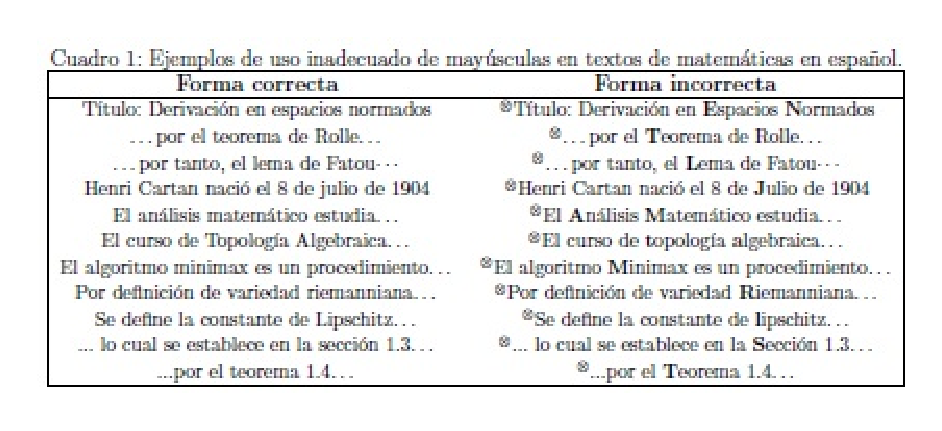
\includegraphics[width=14.5cm]{gutu.eps}
   \caption{Tabla tomada de \cite{MR3052697}}\label{gutu}
\end{center}
\end{figure}
%%%%%%%%%%%%%%%%%%%%%%%%%%%%%%%
%
\subsection{Cap\'itulos y ap\'endices}
Los cap\'itulos se enumeran con un n\'umero ar\'abigo y se recomienda incluir una mini-p\'agina con una descripci\'on del respectivo cap\'itulo.
Los ap\'endices se ordenan con letras may\'usculas $A, B, C \dots$ y debe aparecer en el contenido.
\par
Los niveles que se deben considerar son cap\'itulo, secci\'on, subsecci\'on y p\'arrafo; los cuales deben incluir lemas, proposiciones, teoremas y colorarios. Adem\'as, vale la pena ilustrar la exposici\'on  con \'utiles ejemplos.
Una herramienta que enriquece la redacci\'on consiste en enumerar los p\'arrafos no solo para citarlos y simplificar la exposici\'on, sino tambi\'en  para incluir solo aquellos que son necesarios en la redacci\'on clara y concisa del trabajo de tesis.
%
\begin{obs}
Para ilustrar el uso se escribe a modo de observación que las modificiones de la nueva carátula ya no incluyen el nombre de los jurados.
Sin embargo, estas deben aparecer en la hoja de presentación y para citar el nombre de cada uno se debe tener en cuenta la p\'agina \textsc{orcid} de cada integrante el jurado.
Consulte \texttt{https://orcid.org/} o bien \texttt{https://www.scopus.com/freelookup/form/author.uri}
\end{obs}
%
Las conclusiones aparecen al final con el comando \texttt{chapter*} y debe aparecer en el \'indice general.
\subsection{Bibliograf\'ia}%
La bibliograf\'ia se recomienda usar BibTEX en el estilo \texttt{amsalpha}, que produce etiquetas usando el nombre del autor y el a\~{n}o de la publicaci\'on.
El estilo \texttt{amsplain} genera números, pero en ambos casos se genera de modo automático sólo la bibliografia citada y con la información precisa para ubicarla en la literatura.

\pretolerance=20000\tolerance=30000
\selectlanguage{spanish}
\pagestyle{fancy}
\chapter[Guía para formato y citado de documentos de tesis]{Guía para formato y citado de documentos de tesis y trabajos de investigación – Escuela de Posgrado}\label{cap:2}
\vspace*{1cm}
\begin{center}
\begin{minipage}{12cm}
%------------------------------------------------
\texttt{\baselineskip 10pt
\begin{flushright}
pude introducir una cita\\
de su elecci\'on.\\
{\sf Autor de la cita.}
\end{flushright}}
%-------------------------------------
\textsl{\baselineskip 10pt
A modo de ejemplo en el empledo de la plantilla se \textbf{transcribe} todo el documento intitulado <<Guía para formato y citado de documentos de tesis y trabajos de investigación – Escuela de Posgrado>> que se encuentra en intranet. Las recomendaciones del primer capítulo son las adecuadas para el programa y se construyeron siguiendo parte de la guia. La carátula y el resumen que cita la guia es la que se utiliza en el presente formato}
\end{minipage}
\end{center}

\bigskip
La siguiente es una guía con una lista de recomendaciones para la elaboración de los documentos de tesis y trabajos de investigación. Esta lista no se considera exhaustiva, por lo que el cumplimiento de estas recomendaciones no excluye la posibilidad de que su documento sea observado por alguna causa no contemplada en la misma.

\section{En materia de formato}%
Sobre la Carátula:
\begin{itemize}
  \item Sírvase utilizar la plantilla de Carátula \index{Car\'atula} adjunta a este documento, prestando atención a reemplazar todo texto entre corchetes -- incluyendo los corchetes -- con la información correspondiente a su documento de tesis y programa. \\
      \emph{Nota:} Algunas tesis requieren de la utilización de carátulas específicas, las cuáles pueden emplear según lo indicado por su programa.
  \item No numere su Carátula.
\end{itemize}
Sobre el Resumen:
\begin{itemize}
  \item Su documento de tesis debe contar con un Resumen.
  \item Las pautas para la elaboración del Resumen se encuentran junto con la plantilla de carátula.
  \item La ubicación recomendada para el Resumen es en la página inmediatamente siguiente a la Carátula.
  \item La extensión ideal para el resumen es de 200-300 palabras; se aceptarán resúmenes de hasta una página de extensión.
\end{itemize}
Sobre el Índice:
\begin{itemize}
  \item Es necesario que el Índice indique las páginas del cuerpo de su tesis correspondientes a las secciones que menciona.
  \item Es necesario que el Índice mencione las páginas correctas. Sírvase revisar que este sea el caso, y corregir su Índice si realiza alguna modificación al cuerpo de su tesis que altere su cantidad de páginas o el orden de las secciones.
\end{itemize}
Indicaciones generales:
\begin{itemize}
  \item No utilice páginas en blanco o <<de respeto>>.
  \item No utilice encabezados ni pies de página mencionando su nombre, el título de la tesis, la sección o capítulo, etc (para matem\'aticas se ha modificado).
  \item No utilice marcas de agua.
  \item No entregue su documento con resaltados y comentarios.
  \item Su documento debe ser entregado en formato PDF.
  \item Debe entregar un solo archivo para su revisión; no está permitido entregar la tesis y los anexos en archivos separados.
\end{itemize}

\section{En materia de citado}%
Sobre la revisión de su documento:
\begin{itemize}
  \item La EP no se encargará de realizar revisiones de su documento de tesis previas a su revisión formal. Para este fin, cada programa tiene acceso a una cuenta de Turnitin, con la cual puede revisar su documento.
\end{itemize}
Sobre las citas textuales:
\begin{itemize}
  \item Toda cita textual deberá hacer un uso adecuado de comillas o de sangría, acorde a su extensión.
  \item \textit{Modificar las primeras palabras de un párrafo y/o reemplazar algunos verbos, sustantivos o adjetivos por sus sinónimos no convierte un extracto textual en una paráfrasis. Los extractos que sigan este patrón de modificación serán tratados como citas textuales, y será requerido un citado acorde.}
  \item Si tiene dudas adicionales sobre citado, puede usar como referencia la Guía {\sc pucp} disponible en el siguiente enlace:\\
      \emph{\small http://files.pucp.edu.pe/homepucp/uploads/2016/06/08105745/Guia$\_$PUCP$\_$ para$\_$el$\_$registro$\_$y$\_$citado$\_$de$\_$fuentes-2015.pdf}\\
      En particular, el citado para extractos textuales y paráfrasis se encuentra en las pp. 83 y 84 del documento.
\end{itemize}
%%%%%%%%%%%%%%%%%%%%%%%%%%%%%%%%%%%%%%%%%%%%%%%%%%%%%%%%%%%%%%%%%%%%%%%%%%%%%%%%%%%%%%%%
%%%%
%%%%-----------------------------CONCLUSION-----------------------------------------------
%%%%
%%%%%%%%%%%%%%%%%%%%%%%%%%%%%%%%%%%%%%%%%%%%%%%%%%%%%%%%%%%%%%%%%%%%%%%%%%%%%%%%%%%%%%%%%
\selectlanguage{spanish}
\chapter*{Conclusiones}\addcontentsline{toc}{chapter}{Conclusiones}%
%
Incluya las conclusiones finales del trabajo.
%
\begin{itemize}
  \item El principal resultado\dots
  \item De acuerdo al cap\'itulo \dots
\end{itemize}

\pretolerance=20000\tolerance=30000
\selectlanguage{spanish}
\pagestyle{fancy}
\chapter[Tercer cap\'itulo]{El Teorema de Hodge}\label{cap:3}
\vspace*{1cm}
\begin{center}
\begin{minipage}{12cm}
%------------------------------------------------
\texttt{\baselineskip 10pt
\begin{flushright}
pude introducir una cita\\
de su elecci\'on.\\
{\sf Autor de la cita.}
\end{flushright}}
%-------------------------------------
\textsl{\baselineskip 10pt
El objetivo de este capítulo es demostrar el Teorema de descomposición de Hodge. Este dice que toda k-forma sobre una variedad riemanniana compacta se puede escribir como la suma de una componente $\alpha$, solución de la ecuación $\Delta \alpha = \omega$, donde $\Delta$ es el operador de Laplace-Beltrami, y una componente armónica (en el núcleo de $\Delta$). Como corolario de este teorema se verá además que existe una única forma armónica para cada clase de cohomología. La demostración de este teorema es extensa y hace uso de de la teoría de operadores elípticos y de espacios de Sobolev.}
\end{minipage}
\end{center}

\section{El operador de Laplace-Beltrami}%






%
\section{Espacios de Sobolev}%
%

\begin{defi} Sea $S$ el espacio vectorial complejo de sucesiones de vectores en $\mathbb{C}^m$ con índice dado por una n-tupla $\xi = (\xi_1, \ldots, \xi_n)$. Dado un entero $s$, el espacio de Sobolev $H_s$ es el subespacio de $S$ dado por
\[H_s = \{u \in S: \sum_\xi (1+|\xi|^2)^s\,|u_\xi|^2 < \infty\}\].
\end{defi}






\section{Operadores elípticos}%
%
\begin{defi}
Sea $L$ un operador diferencial parcial de orden $l$. escribimos $L$ como
\[L = P_1(D) + \ldots + P_l(D)\].
Donde $P_j(D)$ es una matriz $m \times m$, que tiene en cada una de sus entradas un operador diferencial $\sum\limits_{[\alpha] = j}a_\alpha D^\alpha$, homogéneo de orden $j$, y donde los $a_\alpha$ son funciones $C^\infty$ sobre $\mathbb{R}$ con valores en $\mathbb{C}$.\\
Denótese $P_j(\xi)$ la matriz obtenida al sustituir $\xi^\alpha$ para $D^\alpha$ en $P_j(D)$, donde $\xi = (\xi_1, \ldots, \xi_n)$ es un punto en $\mathbb{R}^n$. Se dice que $L$ es \textbf{elíptico en el punto x} $\in \mathbb{R}$ si la matriz $P_j(\xi)$ es no singular en x para todo $\xi \neq 0$. L es \textbf{elíptico} si es elíptico en todo $x$.
\end{defi}


\begin{lem} Un operador diferencial parcial $L$ es elíptico si y solo si,para todo $x \in M$, toda función $C^\infty$ $\phi\colon M \to \mathbb{R}$ con $\phi(x) = 0$ y $d\phi(x) \neq 0$ y toda forma $\alpha$ en $M$ se tiene
\begin{equation}
    \Delta(\phi^2\alpha)(x) \neq 0
\end{equation}
\end{lem}
\begin{proof}
Poo poo pee pee
\end{proof}








%
\subsection{Elipticidad del operador de Laplace-Beltrami}%

Resta un último ingrediente para la finalizar la demostración del Teorema de Hodge: la prueba de que, como se aseguró previamente, este es un operador elíptico. Con este fin, se presentan los siguientes lemas.\\
\begin{lem}
Sea  \( U \xrightarrow{\text{T}} V \xrightarrow{\text{S}} W\) una secuencia exacta de espacios vectoriales con producto interno, donde $T^{*}\colon V \to U$ y $S^{*}\colon W \to V$ son las aplicaciones adjuntas de T y S respectivamente. Entonces \(S^{*}S+TT^{*}\) es un isomorfismo.
\end{lem}

\begin{proof}
Sea $v\in V$ diferente de 0, se mostrará que $S^{*}S+TT^{*}$ es diferente de 0. Se tiene que \[\langle (S^{*}S+TT^{*})v,v\rangle = \langle S^{*}Sv, v\rangle + \langle TT^{*}v, v\rangle = \langle Sv, Sv\rangle + \langle T^{*}v, T^{*}v\rangle = \|Sv\|^2+\|Tv\|^2,\]\
Entonces, si $Sv \neq 0$, $\|Sv\|^2+\|T^{*}v\|^2 > 0$.

Si $Sv = 0$, $v\in \text{im} S$, y como la secuencia es exacta, $v\in \text{im}T$. Nótese, por otro lado, que $T^{*}$ es inyectivo en $\text{im}T$ (pues, si $T^{*}w = 0$, para $w = Tu$, para algún $u\in V$, entonces $\langle Tu,Tu \rangle = 0$ y $w = Tu = 0$). De ahí se obtiene que $T^{*}v \neq 0$, lo que implica, de nuevo, que $\|Sv\|^2+\|T^{*}v\|^2 > 0$.\\
\end{proof}

Sea $\hat\xi\colon\bigwedge T_xM \to
\bigwedge T_xM$ la aplicación lineal dada por $\hat\xi\, (\omega) = \xi \wedge \omega$, para $\xi\in T^{*}_xM$, y sea $\hat\xi_l$ su restricción a ${\bigwedge^k T_xM}$. El lema anterior será aplicado a la secuencia de espacios vectoriales
\begin{equation}
\label{secuencia}
\bigwedge^{k-1}T_xM \xrightarrow{\hat\xi_{k-1}}
\bigwedge^{k}T_xM \xrightarrow{\hat\xi_k}\bigwedge^{k+1}T_xM
\end{equation}

Estos espacios vectoriales tienen un producto interno dado por \[ \langle \eta,\omega\rangle = \star(\eta \wedge \star\omega)\]
Esta expresión resulta de aplicar la estrella de Hodge a ambos lados de 
$\eta \wedge \star\omega = \langle \eta,\omega\rangle \text{vol} $ y del hecho que $\star \text{vol} = 1$.
Por supuesto, primero se debe verificar que dicha secuencia sea exacta.

\begin{lem}
La secuencia (\ref{secuencia}) es exacta.
\end{lem}

\begin{proof}
Debido a que $\xi \wedge \xi \wedge \omega = 0$,   para algún $\xi \wedge \omega$ en $\text{im}\, \xi_{k-1}$, se tiene que también pertenece a $\ker \xi_{k}$.\\
Para la otra inclusión se considera el producto interno previamente definido en $\bigwedge^{k}T_xM$. Se toma una base ortonormal $\{\phi_1,\phi_2, \ldots,\phi_n\}$ y se elige $\phi_1$ de modo que $\xi = \|\xi\|\,\phi_1$. Como $\eta = \sum{a_I\, \phi_I}$, (donde $I = (i_1, i_2,\ldots,i_k)$ y $\phi_I = \phi_{i_1}\wedge\phi_{i_2}\wedge\ldots\wedge \phi_{i_k}$) se tiene que $\xi \wedge \eta = \sum{a_I\,\xi \wedge \phi_I}$.\\
Si $1 \in I$, $\xi \wedge \phi_I = \|\xi\|\,\phi_1 \wedge \phi_1 \wedge \ldots \wedge \phi_{i_k} = 0$. En caso contrario, $\xi \wedge \phi_I = \|\xi\|\,\phi_1\wedge\phi_I$, que es múltiplo de un elemento de la base de $\bigwedge^{k+1}T_xM$. De estas observaciones, $\xi \wedge \eta = \sum{a_I\,\xi \wedge \phi_I}$ es combinación lineal de elementos de la base de $\bigwedge^{k+1}T_xM$. Como $\xi \wedge \eta = 0$, por independencia lineal, cada elemento de la suma debe ser igual a 0, lo que solo puede ocurrir si $\phi_1 = \xi / \|\xi\|$ es un factor de $\phi_I$, para todo I y por tanto un factor de $\eta$. Es decir, si $\eta = \xi \wedge \nu $, para algún $\nu$.   
\end{proof}

\begin{lem}
La adjunta de $\hat\xi_k\colon\bigwedge^{k}T_xM\to\bigwedge^{k+1}T_xM$ es
\[(-1)^{nk}\star\hat\xi\,\star\colon \bigwedge^{k+1}T_xM \to \bigwedge^{k}T_xM\]
\end{lem}

\begin{proof}
De las propiedades básicas de la estrella de Hodge se tiene:
\begin{align*}
    \langle \hat \xi_k\,\eta, \omega \rangle = \langle \xi \wedge \eta, \omega\rangle = \star(\xi \wedge \eta \wedge\star\omega) &= (-1)^k\star(\eta \wedge \xi\wedge\star\omega)\\ &= (-1)^k(-1)^{k(n-p)}\star(\eta \wedge  \star\star(\hat\xi\star\omega)) \\
    &= (-1)^{nk}\langle\eta, \star(\hat\xi\star\omega)\rangle
\end{align*}
Así, $(-1)^{nk}\star\hat\xi\star$ es la adjunta de $\hat\xi_k$
\end{proof}


De los tres lemas previos, se obtiene que
\begin{equation}
\label{isomorfismo}
    (-1)^{nk}\star\hat\xi\star\hat\xi + (-1)^{n(k-1)}\hat\xi\star\hat\xi\star
\end{equation}
es un isomorfismo sobre $\bigwedge^{k}T_xM$.
\\

Ahora, se vio anteriormente que un operador diferencial parcial sobre una variedad $M$ es elíptico si y solo si, para todo $x \in M$, toda función $\phi\colon M \to \mathbb{R}$ de clase $C^\infty$ con $\phi(x) = 0$ y $d\phi(x) \neq 0$ y toda forma $\alpha$ en $M$ se tiene
\begin{equation}
\label{eliptico}
    \Delta(\phi^2\alpha)(x) \neq 0
\end{equation}

Sea $\alpha$ una k-forma y $d\phi(x) \neq 0 = \xi \in T^*_xM$ y recuérdese que la estrella de Hodge está dada por:
\[\Delta  = (-1)^{nk+1}\star d \star d + (-1)^{n(k+1)+1}d\star d\star \]

Aplicando esta fórmula en (\ref{eliptico}) obtenemos, primero, para el primer término:
\begin{align*}
\star d\star d(\phi^2 \alpha) &= \star d\star (2\phi\, d\phi\wedge \alpha + \phi^2 d\alpha) \\ 
&= \star d (2\phi \star (d\phi\wedge \alpha) + \phi^2 \star d\alpha) \\
&= \star (2d\phi \wedge \star (d\phi\wedge \alpha) + \cancel{2\phi\, d \star (d\phi\wedge \alpha)} + \cancel{d(\phi^2 \star d\alpha)})\\
&= 2\star \hat\xi \star (\hat\xi\,\alpha)
\end{align*}

Y para el segundo término:
\begin{align*}
d\star d\star(\phi^2 \alpha) &= d\star d(\phi^2 \star\alpha)
= d\star (2\phi\, d\phi\wedge \star\alpha + \phi^2 d(\star\alpha)) \\
&= d (2\phi \star (d\phi\wedge \star\alpha) + \phi^2 \star d(\star\alpha)) \\
&= 2d\phi \wedge \star (d\phi\wedge \star\alpha) + \cancel{2\phi\, d \star (d\phi\wedge \star\alpha)} + \cancel{d(\phi^2 \star d(\star\alpha))}\\
&= 2\hat\xi \star (\hat\xi \star\alpha)
\end{align*}

En el punto $x$, se tiene, entonces:
\begin{equation}
    \Delta(\phi^2\alpha)(x) = -2[(-1)^{nk}\star \hat\xi \star \hat\xi+(-1)^{n(k-1)}\hat\xi \star \hat\xi \star](\alpha(x))
\end{equation}
\\
Como el término entre corchetes es el isomorfismo (\ref{isomorfismo}), hallado gracias a los lemas, y como $\alpha(x) \neq 0$, entonces $\Delta(\phi^2\alpha)(x) \neq 0$. \textbf{Es decir, $\Delta$ es elíptico}.


\section{Demostración final}%

\begin{teo}[Regularidad]
Sea $\alpha_n \in \Omega^k(M)$ y sea $l$ una solución débil de $\Delta\omega = \alpha$. Entonces existe $\omega \in \Omega^k(M)$ tal que
\[l(\beta) = \langle \omega, \beta\rangle\]
para todo $\beta \in \Omega^k(M)$. Por lo tanto, $\Delta\omega = \alpha$.
\end{teo}


\begin{teo}
Sea $\{\alpha_n\}$ una sucesión de k-formas en M tales que $\|\alpha_n\| \leq c$ y $\|\Delta\alpha_n\| \leq c$ para todo $n$ y para alguna constante $c > 0$. Entonces, existe una subsucesión de $\{\alpha_n\}$ que es sucesión de Cauchy en $\Omega^k(M)$.
\end{teo}


Con esto, tenemos ahora una versión puramente analítica del teorema \ref{}:


\begin{teo}[Regularidad]
Dado $p \in \mathbb{R}^n$, existe una vecidad $U_p$ de $p$ y un elemento $u_p$ de $\mathcal{P}$ tales que $l(\phi) = \langle u_p, \phi\rangle$, para todo $\phi \in C_0^\infty(U_p)$
\end{teo}

\begin{proof}

\end{proof}



%
\section{Consecuencias}%
A continuación se utilizará el Teorema de Hodge para la demostración de algunos teoremas.
\pretolerance=20000\tolerance=30000
\selectlanguage{spanish}
\pagestyle{fancy}
\chapter[Tercer cap\'itulo]{Tópicos Adicionales}\label{cap:4}
\vspace*{1cm}
\begin{center}
\begin{minipage}{12cm}
%------------------------------------------------
\texttt{\baselineskip 10pt
\begin{flushright}
pude introducir una cita\\
de su elecci\'on.\\
{\sf Autor de la cita.}
\end{flushright}}
%-------------------------------------
\textsl{\baselineskip 10pt
BLABLABLABLBALBALBLABLABALBALBALBALBABLALBA LALABLABALBABALBABAB LABLABLABLABALABLABLABALBALBLABALBLABLABLLABL ABLBALBALBALBALBALBALBALBALBABLABLABALBBALBAL}
\end{minipage}
\end{center}

\section{Autovalores y autofunciones}

\section{Complejo de de Rham}

\section{}





%%%%%%%%%%%%%%%%%%%%%%%%%%%%%%%%%%%%%%%%%%%%%%%%%%%%%%%%%%%%%%%%%%
%\include{apendice1}
%---------------------------------referencias
%\pagestyle{plain}
\addcontentsline{toc}{chapter}{Bibliograf\'ia}
%\bibliographystyle{amsplain}
\bibliographystyle{amsalpha}
\bibliography{referenciasTesis}
\newpage%%%%---------------------------------------------------------------------index
\selectlanguage{spanish}
\clearpage
\addcontentsline{toc}{chapter}{\'Indice}
\backmatter
\printindex
\end{document}
